\documentclass[11pt]{article}
\usepackage{mathblatt}


\begin{document}
\pruefheftstil{Wahrscheinlichkeit}{Prüfungsheft P10 \textperiodcentered{} schwach}
\noindent{\Large\bfseries Wahrscheinlichkeit}\hfill{\small\color{mbgrau}Prüfungsheft P10 \textperiodcentered{} schwach}\par\medskip
\pfrueckblick
\begin{pfnr}{}{1.}{}
Kürze $\tfrac{6}{8}$ und schreibe den Bruch als Prozentsatz.
\rechenraster{1}
\fusshilfe{\mbox{1:~$75\,\%$}}
\end{pfnr}
\begin{pfnr}{}{2.}{}
Kürze $\tfrac{3}{6}$ und schreibe den Bruch als Prozentsatz.
\rechenraster{1}
\fusshilfe{\mbox{2:~$50\,\%$}}
\end{pfnr}
\begin{pfnr}{}{3.}{}
Berechne $\tfrac{1}{3}$ von 9 Kugeln.
\fusshilfe{\mbox{3:~3 Kugeln}}
\end{pfnr}
\begin{pfnr}{}{4.}{}
Berechne 50\,\% von 8 Feldern.
\fusshilfe{\mbox{4:~4 Felder}}
\end{pfnr}
\begin{pfnr}{}{5.}{}
Tim wirft 8-mal auf den Korb und trifft 4-mal. Wie groß ist die relative Häufigkeit der Treffer?
\rechenraster{1}
\fusshilfe{\mbox{5:~$0{,}5$}}
\end{pfnr}
\begin{pfnr}{}{6.}{}
Eine Münze wird 50-mal geworfen, 30-mal fällt Zahl. Wie groß ist die relative Häufigkeit für Zahl?
\rechenraster{1}
\fusshilfe{\mbox{6:~$0{,}6$}}
\end{pfnr}
\begin{pfnr}{}{7.}{}
Lose tragen die Nummern 1 bis 60. Wie viele Lose sind es?
\fusshilfe{\mbox{7:~60 Lose}}
\end{pfnr}
\begin{pfnr}{}{8.}{}
Im Kino sind die Plätze 11 bis 19 frei. Wie viele Plätze sind das?
\fusshilfe{\mbox{8:~9 Plätze}}
\end{pfnr}
\begin{pfnr}{}{9.}{}
Berechne $\tfrac{1}{2} \cdot \tfrac{1}{3}$.
\fusshilfe{\mbox{9:~$\tfrac{1}{6}$}}
\end{pfnr}
\begin{pfnr}{}{10.}{}
Berechne $\tfrac{1}{5} + \tfrac{2}{5}$.
\fusshilfe{\mbox{10:~$\tfrac{3}{5}$}}
\end{pfnr}
\pfstufekopf[sergebnisseaufzhlen]{Ergebnisse aufzählen}{in 1 der letzten 5 Prüfungen}
\pfgruppe{}
\begin{pfnr}{eigene Aufgabe}{11.}{}
Paul hat zwei Mützen, eine graue und eine grüne. Er hat zwei Schals, einen gelben und einen weißen. Schreibe alle Paare aus Mütze und Schal auf. Beginne mit den Paaren mit der grauen Mütze.
\rechenraster{1}
\fusshilfe{\mbox{11:~4 Paare: , , ,}}
\end{pfnr}
\pfgruppe{}
\begin{pfnr}{eigene Aufgabe}{12.}{}
Lena hat 3 Hosen und 2 Pullover. Wie viele Kombinationen aus Hose und Pullover gibt es?
\par\noindent \leerfeld[Kombinationen] \par
\rechenraster{1}
\fusshilfe{\mbox{12:~$6$ Kombinationen}}
\end{pfnr}
\begin{pfnr}{eigene Aufgabe}{13.}{}
Ein Würfel wird zweimal geworfen. Schreibe alle Paare auf, bei denen der zweite Wurf eine 4 zeigt.
\rechenraster{1}
\fusshilfe{\mbox{13:~6 Paare: , , , , ,}}
\end{pfnr}
\pfgruppe{}
\begin{pfnr}{eigene Aufgabe}{14.}{1 BE}
Zwei Glücksräder haben je vier gleich große Felder: links 4, 5, 4, 6, rechts 5, 5, 6, 4. Beide werden gedreht. Man liest erst die linke, dann die rechte Ziffer. Schreibe alle möglichen zweistelligen Zahlen auf.
\rechenraster{1}
\fusshilfe{\mbox{14:~9 Zahlen: 44, 45, 46, 54, 55, 56, 64, 65, 66}}
\end{pfnr}
\begin{pfnr}{P10 ’25}{15.}{1 BE}
Bei einem Spiel werden zwei Scheiben gleichzeitig gedreht. Bleiben sie stehen, liest man an den Pfeilen erst die Ziffer der linken, dann die der rechten Scheibe ab. Im Bild entsteht so die Zahl 12. Alle Sektoren sind gleich groß. Schreib alle Zahlen auf, die beim Drehen entstehen können.
\par\smallskip\noindent 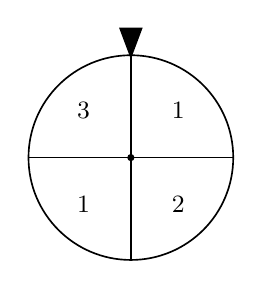
\begin{tikzpicture}[line width=0.6pt,baseline=(current bounding box.north)]\draw (0,0) circle (1.3);\draw (0,0) -- (90:1.3);\node[font=\small] at (45:0.85) {1};\draw (0,0) -- (0:1.3);\node[font=\small] at (-45:0.85) {2};\draw (0,0) -- (-90:1.3);\node[font=\small] at (-135:0.85) {1};\draw (0,0) -- (-180:1.3);\node[font=\small] at (-225:0.85) {3};\fill (0,0) circle (1.3pt);\fill (0,1.25) -- (-0.15,1.65) -- (0.15,1.65) -- cycle;\end{tikzpicture}\hspace{1.2cm}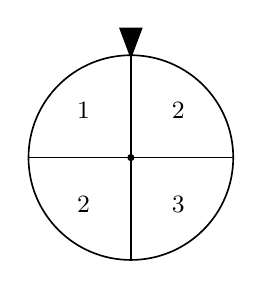
\begin{tikzpicture}[line width=0.6pt,baseline=(current bounding box.north)]\draw (0,0) circle (1.3);\draw (0,0) -- (90:1.3);\node[font=\small] at (45:0.85) {2};\draw (0,0) -- (0:1.3);\node[font=\small] at (-45:0.85) {3};\draw (0,0) -- (-90:1.3);\node[font=\small] at (-135:0.85) {2};\draw (0,0) -- (-180:1.3);\node[font=\small] at (-225:0.85) {1};\fill (0,0) circle (1.3pt);\fill (0,1.25) -- (-0.15,1.65) -- (0.15,1.65) -- cycle;\end{tikzpicture}\par
\rechenraster{1}
\fusshilfe{\mbox{15:~11, 12, 13, 21, 22, 23, 31, 32, 33}}
\end{pfnr}
\begin{pfnr}{eigene Aufgabe}{16.}{2 BE}
Die Ziffern 1, 4 und 7 werden in zufälliger Reihenfolge zu einer dreistelligen Zahl gelegt. Schreibe alle möglichen Zahlen auf. Welcher Anteil davon ist gerade?
\rechenraster{1}
\fusshilfe{\mbox{16:~$\tfrac{1}{3}$}}
\end{pfnr}
\begin{pfnr}{eigene Aufgabe}{17.}{}
Ein Glücksrad mit den Feldern 5, 7 und 9 wird zweimal gedreht. Trage alle Ergebnisse in die Tabelle ein. Die Zeile steht für die erste Drehung, die Spalte für die zweite. Wie viele Ergebnisse sind es?
\par\smallskip\noindent \sachtabelle{lccc}{ & 5 & 7 & 9}{5 & \leerzelle & \leerzelle & \leerzelle \\ 7 & \leerzelle & \leerzelle & \leerzelle \\ 9 & \leerzelle & \leerzelle & \leerzelle}\par
\rechenraster{1}
\fusshilfe{\mbox{17:~9 Ergebnisse: , , , , , , , ,}}
\end{pfnr}
\pfgruppe{}
\begin{pfnr}{eigene Aufgabe}{18.}{}
Eine Münze wird zweimal geworfen. Schreibe alle Ergebnisse auf, bei denen mindestens einmal Kopf fällt.
\rechenraster{1}
\fusshilfe{\mbox{18:~3 Ergebnisse: , ,}}
\end{pfnr}
\pfgruppe{}
\begin{pfnr}{P10 ’17}{19.}{1 BE}
Zwei gleiche Münzen werden zusammen geworfen. Man unterscheidet, ob Zahl (Z) oder Wappen (W) oben liegt. Gib an, wie viele Ergebnisse möglich sind.
\rechenraster{1}
\fusshilfe{\mbox{19:~4 (ZZ, ZW, WZ, WW)}}
\end{pfnr}
\pfgruppe{}
\begin{pfnr}{P10 ’20}{20.}{3 BE}
Wirft man einen Würfel zweimal hintereinander, gibt es 36 verschiedene Augenpaare. Dabei zählen zum Beispiel (2,1) und (1,2) als verschiedene Ergebnisse. Schreib alle Augenpaare auf, bei denen der zweite Wurf eine 2 zeigt. Ermittle die Wahrscheinlichkeit, im zweiten Wurf eine 2 zu würfeln, und gib sie in Prozent an.
\rechenraster{2}
\fusshilfe{\mbox{20:~(1; 2), (2; 2), (3; 2), (4; 2), (5; 2), (6; 2); $\approx$ 16,7 \%}}
\end{pfnr}
\pfstufekopf[swahrscheinlichkeitan]{Wahrscheinlichkeit angeben}{in 2 der letzten 5 Prüfungen}
\pfgruppe{}
\begin{pfnr}{eigene Aufgabe}{21.}{}
Das Glücksrad im Bild hat sechs gleich große Felder. Kreuze an, welcher Anteil der Felder die 2 zeigt. 
\pfkreuzzeile{$\tfrac{1}{3}$}\pfkreuzzeile{$\tfrac{1}{2}$}
\par\smallskip\noindent \kreisdiagramm{1/1,2/1,2/1,2/1,3/1,3/1}\par
\fusshilfe{\mbox{21:~$\tfrac{1}{2}$}}
\end{pfnr}
\begin{pfnr}{eigene Aufgabe}{22.}{}
In einer Lostrommel liegen 30 Nieten und 5 Gewinne. Gesucht ist die Wahrscheinlichkeit für einen Gewinn. Unterstreiche, was möglich und was günstig ist. Rechne nichts.
\par\noindent möglich: \leerfeld , günstig: \leerfeld \par
\rechenraster{1}
\fusshilfe{\mbox{22:~möglich: 35 Lose , günstig: 5 Gewinne}}
\end{pfnr}
\begin{pfnr}{eigene Aufgabe}{23.}{}
Tim dreht ein Glücksrad einmal. Kreuze an, wie viele Stufen der Versuch hat. Rechne nichts. 
\pfkreuzzeile{eine Stufe}\pfkreuzzeile{zwei Stufen}\pfkreuzzeile{drei Stufen}
\fusshilfe{\mbox{23:~eine Stufe}}
\end{pfnr}
\pfgruppe{}
\begin{pfnr}{eigene Aufgabe}{24.}{}
Ein Würfel wird einmal geworfen. Wie groß ist die Wahrscheinlichkeit für eine 4?
\fusshilfe{\mbox{24:~$\tfrac{1}{6}$}}
\end{pfnr}
\pfgruppe{}
\begin{pfnr}{eigene Aufgabe}{25.}{}
Nils sagt: „Beim Würfeln ist eine 6 seltener als eine 1.“ Begründe, ob Nils recht hat.
\rechenraster{1}
\end{pfnr}
\pfgruppe{}
\begin{pfnr}{eigene Aufgabe}{26.}{}
Das Glücksrad im Bild hat sechs gleich große Felder. Wie groß ist die Wahrscheinlichkeit für die 3?
\par\smallskip\noindent \kreisdiagramm{1/1,3/1,2/1,3/1,1/1,3/1}\par
\rechenraster{1}
\fusshilfe{\mbox{26:~$\tfrac{1}{2}$}}
\end{pfnr}
\begin{pfnr}{eigene Aufgabe}{27.}{}
Ein Würfel wird einmal geworfen. Wie groß ist die Wahrscheinlichkeit für eine Zahl kleiner als 3?
\rechenraster{1}
\fusshilfe{\mbox{27:~$\tfrac{1}{3}$}}
\end{pfnr}
\begin{pfnr}{P10 ’14}{28.}{1 BE}
In einer Lostrommel liegen 80 Nieten und 20 Gewinnlose. Gib die Wahrscheinlichkeit P(Gewinn) an.
\rechenraster{1}
\fusshilfe{\mbox{28:~$\tfrac{1}{5}$ = 20 \%}}
\end{pfnr}
\begin{pfnr}{P10 ’14}{29.}{1 BE}
Ein Spielwürfel wird einmal geworfen. Gib die Wahrscheinlichkeit an, dass weder eine 1 noch eine 6 fällt.
\rechenraster{1}
\fusshilfe{\mbox{29:~$\tfrac{2}{3}$}}
\end{pfnr}
\pfgruppe{}
\begin{pfnr}{eigene Aufgabe}{30.}{1 BE}
Drei Dosen enthalten je 8 Bonbons: links 5 Kirsch und 3 Zitrone, in der Mitte 4 Kirsch und 4 Zitrone, rechts 2 Kirsch und 6 Zitrone. Kreuze an, aus welcher Dose man Kirsch mit der Wahrscheinlichkeit 50\,\% zieht. 
\pfkreuzzeile{linke Dose}\pfkreuzzeile{mittlere Dose}\pfkreuzzeile{rechte Dose}
\fusshilfe{\mbox{30:~mittlere Dose}}
\end{pfnr}
\begin{pfnr}{P10 ’15}{31.}{1 BE}
In jedem der drei Töpfe liegen sechs Kugeln. Die Wahrscheinlichkeit, blind eine weiße Kugel zu ziehen, soll 50 \% sein. Kreuze an, aus welchem Topf gezogen werden muss: Topf 1:
\pfkreuzzeile{4 weiße, 2 graue Kugeln}\pfkreuzzeile{Topf 2: 2 weiße, 4 graue Kugeln}\pfkreuzzeile{Topf 3: 3 weiße, 3 graue Kugeln}
\par\smallskip\noindent 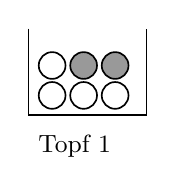
\begin{tikzpicture}[line width=0.6pt]\draw (0,1.1) -- (0,0) -- (1.5,0) -- (1.5,1.1);\draw[fill=white] (0.30,0.25) circle (0.17);\draw[fill=white] (0.70,0.25) circle (0.17);\draw[fill=white] (1.10,0.25) circle (0.17);\draw[fill=white] (0.30,0.63) circle (0.17);\draw[fill=black!40] (0.70,0.63) circle (0.17);\draw[fill=black!40] (1.10,0.63) circle (0.17);\node[font=\small] at (0.75,-0.4) {Topf 1\quad $\square$};\end{tikzpicture}\hspace{0.8cm}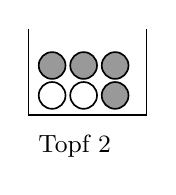
\begin{tikzpicture}[line width=0.6pt]\draw (0,1.1) -- (0,0) -- (1.5,0) -- (1.5,1.1);\draw[fill=white] (0.30,0.25) circle (0.17);\draw[fill=white] (0.70,0.25) circle (0.17);\draw[fill=black!40] (1.10,0.25) circle (0.17);\draw[fill=black!40] (0.30,0.63) circle (0.17);\draw[fill=black!40] (0.70,0.63) circle (0.17);\draw[fill=black!40] (1.10,0.63) circle (0.17);\node[font=\small] at (0.75,-0.4) {Topf 2\quad $\square$};\end{tikzpicture}\hspace{0.8cm}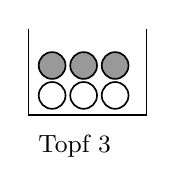
\begin{tikzpicture}[line width=0.6pt]\draw (0,1.1) -- (0,0) -- (1.5,0) -- (1.5,1.1);\draw[fill=white] (0.30,0.25) circle (0.17);\draw[fill=white] (0.70,0.25) circle (0.17);\draw[fill=white] (1.10,0.25) circle (0.17);\draw[fill=black!40] (0.30,0.63) circle (0.17);\draw[fill=black!40] (0.70,0.63) circle (0.17);\draw[fill=black!40] (1.10,0.63) circle (0.17);\node[font=\small] at (0.75,-0.4) {Topf 3\quad $\square$};\end{tikzpicture}\par
\fusshilfe{\mbox{31:~rechter Topf (3 weiße, 3 graue Kugeln)}}
\end{pfnr}
\pfgruppe{}
\begin{pfnr}{eigene Aufgabe}{32.}{2 BE}
Auf einem Teller liegen 18 Muffins, 3 davon mit Chili, die anderen mit Schokolade. Jonas hat schon 2 Schoko-Muffins gegessen. Mara sagt: „Die Wahrscheinlichkeit, jetzt einen Chili-Muffin zu erwischen, ist $\tfrac{3}{18}$.“ Begründe, ob Mara recht hat.
\rechenraster{1}
\end{pfnr}
\pfgruppe{}
\begin{pfnr}{eigene Aufgabe}{33.}{}
In einer Urne liegen 5 rote, 3 blaue und 1 grüne Kugel. Eine Kugel wird gezogen. Wie groß ist die Wahrscheinlichkeit für Blau?
\rechenraster{1}
\fusshilfe{\mbox{33:~$\tfrac{1}{3}$}}
\end{pfnr}
\begin{pfnr}{eigene Aufgabe}{34.}{1 BE}
In einer Schachtel liegen 50 Murmeln: 18 blaue, 9 rote und 23 grüne. Eine Murmel wird gezogen. Wie groß ist die Wahrscheinlichkeit für Rot als Bruch, als Dezimalzahl und in Prozent?
\rechenraster{1}
\fusshilfe{\mbox{34:~$18\,\%$}}
\end{pfnr}
\begin{pfnr}{eigene Aufgabe}{35.}{1 BE}
Bei einer Tombola liegen 45 Nieten und 15 Gewinnlose in der Trommel. Wie groß ist die Wahrscheinlichkeit für einen Gewinn?
\rechenraster{1}
\fusshilfe{\mbox{35:~$\tfrac{1}{4}$}}
\end{pfnr}
\begin{pfnr}{P10 ’16}{36.}{1 BE}
Von 100 Energiesparlampen in einer Kiste sind 5 defekt. Eine Lampe wird herausgenommen. Gib die Wahrscheinlichkeit an, dass sie defekt ist.
\rechenraster{1}
\fusshilfe{\mbox{36:~$\tfrac{1}{20}$ = 5 \%}}
\end{pfnr}
\begin{pfnr}{P10 ’19}{37.}{1 BE}
In einer Kiste liegen 20 Buntstifte: 7 grüne, 4 rote, 3 gelbe und 6 blaue. Paul greift blind einen Stift heraus und legt ihn danach zurück. Gib die Wahrscheinlichkeit an, dass er einen gelben Stift gegriffen hat.
\rechenraster{1}
\fusshilfe{\mbox{37:~$\tfrac{3}{20}$ = 15 \%}}
\end{pfnr}
\begin{pfnr}{P10 ’24}{38.}{1 BE}
In Familie Siebert helfen alle 5 Kinder im Haushalt. Jede Aufgabe steht auf einem Zettel: Müll rausbringen, Spülmaschine ausräumen, Staubsaugen, Einkaufen, Joker. Wer den Joker hat, hat die Woche frei. Zu Wochenbeginn zieht jedes Kind zufällig genau einen Zettel. Gib die Wahrscheinlichkeit an, dass das erste Kind den Zettel „Staubsaugen“ zieht.
\rechenraster{1}
\fusshilfe{\mbox{38:~$\tfrac{1}{5}$ = 20 \%}}
\end{pfnr}
\begin{pfnr}{P10 ’17}{39.}{2 BE}
An einem Zahlenschloss lässt sich jeder der drei Ringe auf eine Ziffer von 0 bis 9 stellen. Jan stellt die ersten beiden Ringe richtig ein. Die Ziffer für den dritten Ring weiß er nicht mehr. Gib als Bruch und in Prozent an, mit welcher Wahrscheinlichkeit er sie beim ersten Versuch trifft.
\rechenraster{1}
\fusshilfe{\mbox{39:~$\tfrac{1}{10}$ = 10 \%}}
\end{pfnr}
\pfgruppe{}
\begin{pfnr}{eigene Aufgabe}{40.}{}
Die Gewinnwahrscheinlichkeit beträgt 35\,\%. Schreibe sie als gekürzten Bruch und als Dezimalzahl.
\rechenraster{1}
\fusshilfe{\mbox{40:~$0{,}35$}}
\end{pfnr}
\pfgruppe{}
\begin{pfnr}{P10 ’16}{41.}{2 BE}
Mia und Lukas verkaufen Lose mit den Nummern 101 bis 900, jede Nummer genau einmal. Gezogen wird die Nummer 326. Den Hauptgewinn bekommt das Los 326. Einen Trostpreis bekommt jedes Los, das auf 26 endet, aber nicht die 326 ist. Mit einem einzigen Los gewinnt man den Hauptgewinn mit der Wahrscheinlichkeit $\tfrac{1}{800}$. Begründe das.
\par\smallskip\noindent \fbox{\parbox{6cm}{\small\textbf{Gewinnplan}\\ Hauptgewinn: Los-Nr.\ 326\\ Trostpreis: alle Lose mit der Endung 26 (außer 326)}}\par
\rechenraster{1}
\fusshilfe{\mbox{41:~900 $-$ 101 + 1 = 800 Lose, 1 Hauptgewinn $\Rightarrow$ $\tfrac{1}{800}$}}
\end{pfnr}
\pfgruppe{}
\begin{pfnr}{P10 ’14}{42.}{2 BE}
Für ein Kinderfest hat Pauls Vater ein Glücksrad gebaut. In einer Spielrunde wird es zweimal nacheinander gedreht. Alle Felder sind gleich groß und werden gleich wahrscheinlich getroffen. Ermittle die Wahrscheinlichkeit, dass der Zeiger auf ein B zeigt. Gib das Ergebnis als Bruch und in Prozent an.
\par\smallskip\noindent 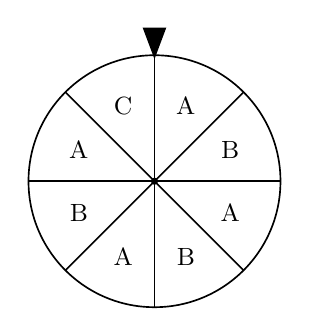
\begin{tikzpicture}[line width=0.6pt,baseline=(current bounding box.north)]\draw (0,0) circle (1.6);\draw (0,0) -- (90:1.6);\node[font=\small] at (67.5:1.04) {A};\draw (0,0) -- (45:1.6);\node[font=\small] at (22.5:1.04) {B};\draw (0,0) -- (0:1.6);\node[font=\small] at (-22.5:1.04) {A};\draw (0,0) -- (-45:1.6);\node[font=\small] at (-67.5:1.04) {B};\draw (0,0) -- (-90:1.6);\node[font=\small] at (-112.5:1.04) {A};\draw (0,0) -- (-135:1.6);\node[font=\small] at (-157.5:1.04) {B};\draw (0,0) -- (-180:1.6);\node[font=\small] at (-202.5:1.04) {A};\draw (0,0) -- (-225:1.6);\node[font=\small] at (-247.5:1.04) {C};\fill (0,0) circle (1.3pt);\fill (0,1.55) -- (-0.15,1.95) -- (0.15,1.95) -- cycle;\end{tikzpicture}\par
\pfzwfrage{Zähle die Felder mit B.}
\rechenraster{2}
\fusshilfe{\mbox{42:~$\tfrac{3}{8}$; 37,5 \%}}
\end{pfnr}
\pfgruppe{}
\begin{pfnr}{P10 ’18}{43.}{2 BE}
Eva hat 16 Pfannkuchen gebacken: 14 mit Marmelade, 2 mit Senf; von außen sieht man die Füllung nicht. Tom nimmt sich zuerst zwei, beide mit Marmelade. Pia sagt: „Jetzt greift man mit der Wahrscheinlichkeit $\tfrac{2}{16}$ einen Senf-Pfannkuchen.“ Entscheide, ob Pia recht hat, und begründe.
\rechenraster{1}
\fusshilfe{\mbox{43:~nein, P = $\tfrac{2}{14}$ = $\tfrac{1}{7}$ $\approx$ 14,3 \%, nicht $\tfrac{2}{16}$}}
\end{pfnr}
\pfgruppe{}
\begin{pfnr}{P10 ’16}{\llap{\textasteriskcentered\,}44.}{3 BE}
Mia und Lukas verkaufen Lose mit den Nummern 101 bis 900, jede Nummer genau einmal. Gezogen wird die Nummer 326. Den Hauptgewinn bekommt das Los 326. Einen Trostpreis bekommt jedes Los, das auf 26 endet, aber nicht die 326 ist. Anne hat ein Los gekauft. Beim Öffnen sieht sie zuerst nur die letzte Ziffer: eine 6. Sie sagt: „Meine Chance auf einen Trostpreis liegt jetzt bei $\tfrac{7}{80}$.“ Hat Anne recht? Begründe.
\par\smallskip\noindent \fbox{\parbox{6cm}{\small\textbf{Gewinnplan}\\ Hauptgewinn: Los-Nr.\ 326\\ Trostpreis: alle Lose mit der Endung 26 (außer 326)}}\par
\pfzwfrage{Zähle die Lose, die auf 6 enden.}
\rechenraster{3}
\fusshilfe{\mbox{44:~$\tfrac{7}{80}$}}
\end{pfnr}
\pfstufekopf[sbaumergnzen]{Baum ergänzen}{in 2 der letzten 5 Prüfungen}
\pfgruppe{}
\begin{pfnr}{eigene Aufgabe}{45.}{}
In einer Dose sind 9 Kekse, 4 davon mit Schoko. Ein Schokokeks wird gegessen. Wie viele Kekse sind noch da? Wie viele davon sind mit Schoko?
\par\noindent \leerfeld[insgesamt] , davon \leerfeld \par
\rechenraster{1}
\fusshilfe{\mbox{45:~8 Kekse, davon 3 mit Schoko}}
\end{pfnr}
\begin{pfnr}{eigene Aufgabe}{46.}{}
Ein Würfel wird zweimal geworfen. Das Ereignis heißt „mindestens eine Sechs“. Nenne das Gegenereignis.
\rechenraster{1}
\fusshilfe{\mbox{46:~Gegenereignis: keine Sechs in beiden Würfen}}
\end{pfnr}
\begin{pfnr}{eigene Aufgabe}{47.}{}
Ein Glücksrad wird zweimal gedreht. Kreuze an, ob das wie Ziehen mit oder ohne Zurücklegen ist. 
\pfkreuzzeile{mit Zurücklegen}\pfkreuzzeile{ohne Zurücklegen}
\fusshilfe{\mbox{47:~mit Zurücklegen}}
\end{pfnr}
\begin{pfnr}{eigene Aufgabe}{48.}{}
Der Baum zeigt zweimaliges Drehen eines Glücksrads. Schreibe alle Pfade auf, die zum Ereignis „genau einmal Rot“ gehören. Rechne nichts.
\par\smallskip\noindent \baumzwei{rot/,blau/}{rot/,blau/}{rot/,blau/}\par
\rechenraster{1}
\fusshilfe{\mbox{48:~2 Pfade: ,}}
\end{pfnr}
\pfgruppe{}
\begin{pfnr}{eigene Aufgabe}{49.}{}
Ein Glücksrad hat drei gleich große Felder: 1 rotes und 2 blaue. Es wird zweimal gedreht. Trage im Baum an jeden Ast die Wahrscheinlichkeit ein.
\par\smallskip\noindent \baumzwei{rot/,blau/}{rot/,blau/}{rot/,blau/}\par
\rechenraster{1}
\fusshilfe{\mbox{49:~auf beiden Stufen rot $\tfrac{1}{3}$, blau $\tfrac{2}{3}$}}
\end{pfnr}
\begin{pfnr}{eigene Aufgabe}{50.}{}
In einer Urne liegen 3 rote und 5 blaue Kugeln. Zwei Kugeln werden ohne Zurücklegen gezogen. Wie groß ist die Wahrscheinlichkeit für zweimal Rot?
\rechenraster{1}
\fusshilfe{\mbox{50:~$\tfrac{3}{28}$}}
\end{pfnr}
\begin{pfnr}{eigene Aufgabe}{51.}{2 BE}
Ein Glücksrad mit 5 gleich großen Feldern (3-mal grün, 2-mal gelb) wird zweimal gedreht. Im Baum ist nur die Wahrscheinlichkeit für Gelb auf der ersten Stufe eingetragen. Ergänze alle fehlenden Wahrscheinlichkeiten.
\par\smallskip\noindent \baumzwei{\text{grün}/,gelb/\frac{2}{5}}{\text{grün}/,gelb/}{\text{grün}/,gelb/}\par
\rechenraster{1}
\fusshilfe{\mbox{51:~das Glücksrad ändert sich nicht}}
\end{pfnr}
\begin{pfnr}{eigene Aufgabe}{52.}{}
In einem Beutel liegen 4 rote und 3 grüne Kugeln. Zwei werden ohne Zurücklegen gezogen. Ergänze die fehlenden Wahrscheinlichkeiten im Baum.
\par\smallskip\noindent \baumzwei{rot/\frac{4}{7},\text{grün}/}{rot/,\text{grün}/\frac{3}{6}}{rot/,\text{grün}/}\par
\rechenraster{1}
\fusshilfe{\mbox{52:~nach rot: rot $\tfrac{3}{6}$}}
\end{pfnr}
\begin{pfnr}{eigene Aufgabe}{\llap{\textasteriskcentered\,}53.}{}
In einer Schachtel liegen 15 Pralinen, 5 davon mit Nuss. Emil nimmt nacheinander drei Pralinen, ohne zurückzulegen. Ergänze die beiden leeren Felder im Baum.
\par\smallskip\noindent \baumdrei{Nuss/\frac{5}{15},ohne/}{Nuss/\frac{4}{14},ohne/\frac{10}{14}}{Nuss/\frac{5}{14},ohne/\frac{9}{14}}{Nuss/\frac{3}{13},ohne/\frac{10}{13}}{Nuss/\frac{4}{13},ohne/\frac{9}{13}}{Nuss/,ohne/\frac{9}{13}}{Nuss/\frac{5}{13},ohne/\frac{8}{13}}\par
\rechenraster{1}
\fusshilfe{\mbox{53:~erste Stufe ohne Nuss $\tfrac{10}{15}$}}
\end{pfnr}
\pfgruppe{}
\begin{pfnr}{P10 ’24}{54.}{3 BE}
In Familie Siebert helfen alle 5 Kinder im Haushalt. Jede Aufgabe steht auf einem Zettel: Müll rausbringen, Spülmaschine ausräumen, Staubsaugen, Einkaufen, Joker. Wer den Joker hat, hat die Woche frei. Zu Wochenbeginn zieht jedes Kind zufällig genau einen Zettel. Benjamin ist der Jüngste und zieht jede Woche als Erster aus allen fünf Zetteln. Ergänze die Wahrscheinlichkeiten im Baumdiagramm. Benjamin zieht in beiden Wochen den Joker: Weise nach, dass das die Wahrscheinlichkeit $\tfrac{1}{25}$ hat.
\par\smallskip\noindent \begin{tikzpicture}[line width=0.5pt,baseline=(current bounding box.north)]\node[font=\scriptsize,mbgrau] at (2.04,0.70) {1. Woche};\node[font=\scriptsize,mbgrau] at (5.44,0.70) {2. Woche};\fill (0,-1.35) circle (1.3pt) coordinate (k0w);\node[font=\scriptsize,inner sep=2pt] (k0) at (3.40,-2.25) {Joker};\node[font=\scriptsize,inner sep=2pt] (k1) at (3.40,-0.45) {kein Joker};\node[font=\scriptsize,inner sep=2pt] (k5) at (6.80,0.00) {kein Joker};\node[font=\scriptsize,inner sep=2pt] (k2) at (6.80,-2.70) {Joker};\node[font=\scriptsize,inner sep=2pt] (k4) at (6.80,-0.90) {Joker};\node[font=\scriptsize,inner sep=2pt] (k3) at (6.80,-1.80) {kein Joker};\draw[] (k0w) -- node[pos=0.55,anchor=north,draw,line width=0.3pt,fill=white,minimum width=0.7cm,minimum height=0.34cm,inner sep=0pt] {} (k0.west);\draw[] (k0w) -- node[pos=0.55,anchor=south,draw,line width=0.3pt,fill=white,minimum width=0.7cm,minimum height=0.34cm,inner sep=0pt] {} (k1.west);\draw[] (k1.east) -- node[pos=0.55,anchor=south,font=\scriptsize,fill=white,inner sep=1pt] {$\tfrac{4}{5}$} (k5.west);\draw[] (k0.east) -- node[pos=0.55,anchor=north,draw,line width=0.3pt,fill=white,minimum width=0.7cm,minimum height=0.34cm,inner sep=0pt] {} (k2.west);\draw[] (k1.east) -- node[pos=0.55,anchor=north,draw,line width=0.3pt,fill=white,minimum width=0.7cm,minimum height=0.34cm,inner sep=0pt] {} (k4.west);\draw[] (k0.east) -- node[pos=0.55,anchor=south,draw,line width=0.3pt,fill=white,minimum width=0.7cm,minimum height=0.34cm,inner sep=0pt] {} (k3.west);\end{tikzpicture}\par
\pfzwfrage{Gib die Wahrscheinlichkeit an, dass Benjamin in einer Woche den Joker zieht.}
\rechenraster{2}
\fusshilfe{\mbox{54:~1. Woche: kein Joker 4/5, Joker $\tfrac{1}{5}$; $\tfrac{1}{25}$}}
\end{pfnr}
\pfgruppe{}
\begin{pfnr}{eigene Aufgabe}{55.}{}
Der Baum zeigt einen zweistufigen Zufallsversuch. Beschreibe einen Zufallsversuch, der zu diesem Baum passt. Nenne das Gerät, die Beschriftung und wie oft es benutzt wird.
\par\smallskip\noindent \baumzwei{rot/\frac{2}{5},blau/\frac{3}{5}}{rot/\frac{2}{5},blau/\frac{3}{5}}{rot/\frac{2}{5},blau/\frac{3}{5}}\par
\rechenraster{1}
\end{pfnr}
\begin{pfnr}{P10 ’14}{56.}{2 BE}
Für ein Kinderfest hat Pauls Vater ein Glücksrad gebaut. In einer Spielrunde wird es zweimal nacheinander gedreht. Alle Felder sind gleich groß und werden gleich wahrscheinlich getroffen. Trag im Baumdiagramm alle fehlenden Wahrscheinlichkeiten ein.
\par\smallskip\noindent \begin{tikzpicture}[line width=0.5pt,baseline=(current bounding box.north)]\node[font=\scriptsize,mbgrau] at (2.04,0.70) {1. Drehung};\node[font=\scriptsize,mbgrau] at (5.44,0.70) {2. Drehung};\fill (0,-3.80) circle (1.3pt) coordinate (k0w);\node[font=\scriptsize,inner sep=2pt] (k0) at (3.40,-0.95) {A};\node[font=\scriptsize,inner sep=2pt] (k2) at (3.40,-6.65) {C};\node[font=\scriptsize,inner sep=2pt] (k1) at (3.40,-3.80) {B};\node[font=\scriptsize,inner sep=2pt] (k8) at (6.80,-4.75) {C};\node[font=\scriptsize,inner sep=2pt] (k10) at (6.80,-6.65) {B};\node[font=\scriptsize,inner sep=2pt] (k4) at (6.80,-0.95) {B};\node[font=\scriptsize,inner sep=2pt] (k6) at (6.80,-2.85) {A};\node[font=\scriptsize,inner sep=2pt] (k11) at (6.80,-7.60) {C};\node[font=\scriptsize,inner sep=2pt] (k5) at (6.80,-1.90) {C};\node[font=\scriptsize,inner sep=2pt] (k9) at (6.80,-5.70) {A};\node[font=\scriptsize,inner sep=2pt] (k3) at (6.80,0.00) {A};\node[font=\scriptsize,inner sep=2pt] (k7) at (6.80,-3.80) {B};\draw[] (k0w) -- node[pos=0.55,anchor=south,draw,line width=0.3pt,fill=white,minimum width=0.7cm,minimum height=0.34cm,inner sep=0pt] {} (k0.west);\draw[] (k0w) -- node[pos=0.55,anchor=north,font=\scriptsize,fill=white,inner sep=1pt] {$\tfrac{1}{8}$} (k2.west);\draw[] (k0w) -- node[pos=0.55,anchor=south,draw,line width=0.3pt,fill=white,minimum width=0.7cm,minimum height=0.34cm,inner sep=0pt] {} (k1.west);\draw[] (k1.east) -- node[pos=0.55,anchor=north,draw,line width=0.3pt,fill=white,minimum width=0.7cm,minimum height=0.34cm,inner sep=0pt] {} (k8.west);\draw[] (k2.east) -- node[pos=0.55,anchor=south,draw,line width=0.3pt,fill=white,minimum width=0.7cm,minimum height=0.34cm,inner sep=0pt] {} (k10.west);\draw[] (k0.east) -- node[pos=0.55,anchor=north,draw,line width=0.3pt,fill=white,minimum width=0.7cm,minimum height=0.34cm,inner sep=0pt] {} (k4.west);\draw[] (k1.east) -- node[pos=0.55,anchor=south,draw,line width=0.3pt,fill=white,minimum width=0.7cm,minimum height=0.34cm,inner sep=0pt] {} (k6.west);\draw[] (k2.east) -- node[pos=0.55,anchor=north,draw,line width=0.3pt,fill=white,minimum width=0.7cm,minimum height=0.34cm,inner sep=0pt] {} (k11.west);\draw[] (k0.east) -- node[pos=0.55,anchor=north,draw,line width=0.3pt,fill=white,minimum width=0.7cm,minimum height=0.34cm,inner sep=0pt] {} (k5.west);\draw[] (k2.east) -- node[pos=0.55,anchor=south,draw,line width=0.3pt,fill=white,minimum width=0.7cm,minimum height=0.34cm,inner sep=0pt] {} (k9.west);\draw[] (k0.east) -- node[pos=0.55,anchor=south,draw,line width=0.3pt,fill=white,minimum width=0.7cm,minimum height=0.34cm,inner sep=0pt] {} (k3.west);\draw[] (k1.east) -- node[pos=0.55,anchor=north,draw,line width=0.3pt,fill=white,minimum width=0.7cm,minimum height=0.34cm,inner sep=0pt] {} (k7.west);\end{tikzpicture}\par
\rechenraster{1}
\fusshilfe{\mbox{56:~1. Stufe A 1/2, B $\tfrac{3}{8}$; 2. Stufe je Ast A 1/2, B 3/8, C $\tfrac{1}{8}$}}
\end{pfnr}
\pfgruppe{}
\begin{pfnr}{P10 ’19}{\llap{\textasteriskcentered\,}57.}{5 BE}
In einer Kiste liegen 20 Buntstifte: 7 grüne, 4 rote, 3 gelbe und 6 blaue. Marie nimmt aus der vollen Kiste blind nacheinander drei Stifte heraus und legt keinen zurück. Ergänze im Baumdiagramm die Wahrscheinlichkeiten an den zwei leeren Stellen. Entscheide für den fett gezeichneten Pfad, ob die Aussagen wahr oder falsch sind, und kreuze an:
\par\smallskip\noindent \begin{tikzpicture}[line width=0.5pt,baseline=(current bounding box.north)]\node[font=\scriptsize,mbgrau] at (1.80,0.70) {1. Stift};\node[font=\scriptsize,mbgrau] at (4.80,0.70) {2. Stift};\node[font=\scriptsize,mbgrau] at (7.80,0.70) {3. Stift};\fill (0,-2.17) circle (1.3pt) coordinate (k0w);\node[font=\scriptsize,inner sep=2pt] (k0) at (3.00,-3.41) {nicht rot};\node[font=\scriptsize,inner sep=2pt] (k1) at (3.00,-0.93) {rot};\node[font=\scriptsize,inner sep=2pt] (k5) at (6.00,-0.31) {rot};\node[font=\scriptsize,inner sep=2pt] (k2) at (6.00,-4.03) {nicht rot};\node[font=\scriptsize,inner sep=2pt] (k3) at (6.00,-2.79) {rot};\node[font=\scriptsize,inner sep=2pt] (k4) at (6.00,-1.55) {nicht rot};\node[font=\scriptsize,inner sep=2pt] (k12) at (9.00,-0.62) {nicht rot};\node[font=\scriptsize,inner sep=2pt] (k7) at (9.00,-3.72) {rot};\node[font=\scriptsize,inner sep=2pt] (k9) at (9.00,-2.48) {rot};\node[font=\scriptsize,inner sep=2pt] (k10) at (9.00,-1.86) {nicht rot};\node[font=\scriptsize,inner sep=2pt] (k13) at (9.00,0.00) {rot};\node[font=\scriptsize,inner sep=2pt] (k11) at (9.00,-1.24) {rot};\node[font=\scriptsize,inner sep=2pt] (k8) at (9.00,-3.10) {nicht rot};\node[font=\scriptsize,inner sep=2pt] (k6) at (9.00,-4.34) {nicht rot};\draw[] (k0w) -- node[pos=0.55,anchor=north,draw,line width=0.3pt,fill=white,minimum width=0.7cm,minimum height=0.34cm,inner sep=0pt] {} (k0.west);\draw[line width=1.4pt] (k0w) -- node[pos=0.55,anchor=south,font=\scriptsize,fill=white,inner sep=1pt] {$\tfrac{4}{20}$} (k1.west);\draw[line width=1.4pt] (k1.east) -- node[pos=0.55,anchor=south,font=\scriptsize,fill=white,inner sep=1pt] {$\tfrac{3}{19}$} (k5.west);\draw[] (k0.east) --  (k2.west);\draw[] (k0.east) --  (k3.west);\draw[] (k1.east) --  (k4.west);\draw[] (k5.east) --  (k12.west);\draw[] (k2.east) --  (k7.west);\draw[] (k3.east) -- node[pos=0.55,anchor=south,draw,line width=0.3pt,fill=white,minimum width=0.7cm,minimum height=0.34cm,inner sep=0pt] {} (k9.west);\draw[] (k4.east) --  (k10.west);\draw[line width=1.4pt] (k5.east) -- node[pos=0.55,anchor=south,font=\scriptsize,fill=white,inner sep=1pt] {$\tfrac{2}{18}$} (k13.west);\draw[] (k4.east) --  (k11.west);\draw[] (k3.east) --  (k8.west);\draw[] (k2.east) --  (k6.west);\end{tikzpicture}
\par\smallskip\noindent \begingroup\renewcommand{\arraystretch}{1.5}\begin{tabular}{|p{8.0cm}|c|c|}\hline Aussage & wahr & falsch \\ \hline „Marie zieht drei Stifte mit verschiedenen Farben.“ & $\square$ & $\square$ \\ \hline „Marie legt jeden Stift nach dem Ziehen zurück.“ & $\square$ & $\square$ \\ \hline „Der fette Pfad hat eine Wahrscheinlichkeit unter 1 \%.“ & $\square$ & $\square$ \\ \hline\end{tabular}\endgroup\par
\pfzwfrage{Gib an, wie viele rote Stifte vor dem dritten Zug auf dem Pfad nicht rot > rot noch in der Kiste sind.}
\rechenraster{3}
\fusshilfe{\mbox{57:~$\tfrac{16}{20}$; $\tfrac{3}{18}$; Aussage 1 falsch, 2 falsch, 3 wahr}}
\end{pfnr}
\pfgruppe{}
\begin{pfnr}{P10 ’20}{\llap{\textasteriskcentered\,}58.}{3 BE}
Wirft man einen Würfel zweimal hintereinander, gibt es 36 verschiedene Augenpaare. Dabei zählen zum Beispiel (2,1) und (1,2) als verschiedene Ergebnisse. Lisa und Max wollen ins Kino. Lisa würfelt dreimal hintereinander. Fällt dabei mindestens zweimal eine 6, bezahlt Max beide Karten. Vervollständige das Baumdiagramm. Berechne die Wahrscheinlichkeit, dass Max die Karten bezahlt.
\par\smallskip\noindent \begin{tikzpicture}[line width=0.5pt,baseline=(current bounding box.north)]\node[font=\scriptsize,mbgrau] at (1.80,0.70) {1. Wurf};\node[font=\scriptsize,mbgrau] at (4.80,0.70) {2. Wurf};\node[font=\scriptsize,mbgrau] at (7.80,0.70) {3. Wurf};\fill (0,-2.17) circle (1.3pt) coordinate (k0w);\node[font=\scriptsize,inner sep=2pt] (k0) at (3.00,-0.93) {6};\node[font=\scriptsize,inner sep=2pt] (k1) at (3.00,-3.41) {keine 6};\node[font=\scriptsize,inner sep=2pt] (k3) at (6.00,-1.55) {keine 6};\node[font=\scriptsize,inner sep=2pt] (k2) at (6.00,-0.31) {6};\node[font=\scriptsize,inner sep=2pt] (k5) at (6.00,-4.03) {keine 6};\node[font=\scriptsize,inner sep=2pt] (k4) at (6.00,-2.79) {6};\node[font=\scriptsize,inner sep=2pt] (k9) at (9.00,-1.86) {keine 6};\node[font=\scriptsize,inner sep=2pt] (k13) at (9.00,-4.34) {keine 6};\node[font=\scriptsize,inner sep=2pt] (k8) at (9.00,-1.24) {6};\node[font=\scriptsize,inner sep=2pt] (k12) at (9.00,-3.72) {6};\node[font=\scriptsize,inner sep=2pt] (k10) at (9.00,-2.48) {6};\node[font=\scriptsize,inner sep=2pt] (k7) at (9.00,-0.62) {keine 6};\node[font=\scriptsize,inner sep=2pt] (k6) at (9.00,0.00) {6};\node[font=\scriptsize,inner sep=2pt] (k11) at (9.00,-3.10) {keine 6};\draw[] (k0w) -- node[pos=0.55,anchor=south,draw,line width=0.3pt,fill=white,minimum width=0.7cm,minimum height=0.34cm,inner sep=0pt] {} (k0.west);\draw[] (k0w) -- node[pos=0.55,anchor=north,draw,line width=0.3pt,fill=white,minimum width=0.7cm,minimum height=0.34cm,inner sep=0pt] {} (k1.west);\draw[] (k0.east) -- node[pos=0.55,anchor=north,draw,line width=0.3pt,fill=white,minimum width=0.7cm,minimum height=0.34cm,inner sep=0pt] {} (k3.west);\draw[] (k0.east) -- node[pos=0.55,anchor=south,draw,line width=0.3pt,fill=white,minimum width=0.7cm,minimum height=0.34cm,inner sep=0pt] {} (k2.west);\draw[] (k1.east) -- node[pos=0.55,anchor=north,draw,line width=0.3pt,fill=white,minimum width=0.7cm,minimum height=0.34cm,inner sep=0pt] {} (k5.west);\draw[] (k1.east) -- node[pos=0.55,anchor=south,draw,line width=0.3pt,fill=white,minimum width=0.7cm,minimum height=0.34cm,inner sep=0pt] {} (k4.west);\draw[] (k3.east) -- node[pos=0.55,anchor=north,draw,line width=0.3pt,fill=white,minimum width=0.7cm,minimum height=0.34cm,inner sep=0pt] {} (k9.west);\draw[] (k5.east) -- node[pos=0.55,anchor=north,draw,line width=0.3pt,fill=white,minimum width=0.7cm,minimum height=0.34cm,inner sep=0pt] {} (k13.west);\draw[] (k3.east) -- node[pos=0.55,anchor=south,draw,line width=0.3pt,fill=white,minimum width=0.7cm,minimum height=0.34cm,inner sep=0pt] {} (k8.west);\draw[] (k5.east) -- node[pos=0.55,anchor=south,draw,line width=0.3pt,fill=white,minimum width=0.7cm,minimum height=0.34cm,inner sep=0pt] {} (k12.west);\draw[] (k4.east) -- node[pos=0.55,anchor=south,draw,line width=0.3pt,fill=white,minimum width=0.7cm,minimum height=0.34cm,inner sep=0pt] {} (k10.west);\draw[] (k2.east) -- node[pos=0.55,anchor=north,draw,line width=0.3pt,fill=white,minimum width=0.7cm,minimum height=0.34cm,inner sep=0pt] {} (k7.west);\draw[] (k2.east) -- node[pos=0.55,anchor=south,draw,line width=0.3pt,fill=white,minimum width=0.7cm,minimum height=0.34cm,inner sep=0pt] {} (k6.west);\draw[] (k4.east) -- node[pos=0.55,anchor=north,draw,line width=0.3pt,fill=white,minimum width=0.7cm,minimum height=0.34cm,inner sep=0pt] {} (k11.west);\end{tikzpicture}\par
\rechenraster{4}
\fusshilfe{\mbox{58:~Äste 6: 1/6, keine 6: $\tfrac{5}{6}$; $\tfrac{2}{27}$ $\approx$ 7,4 \%}}
\end{pfnr}
\pfgruppe{}
\begin{pfnr}{P10 ’15}{\llap{\textasteriskcentered\,}59.}{4 BE}
Beim Elfmetertraining stehen 11 Spieler bereit. Jeder schießt höchstens einmal; die Reihenfolge wird ausgelost. Die Fans wünschen sich, dass ihr Torjäger Ronny unter den ersten drei Schützen ist. Vervollständige das Baumdiagramm (R: Ronny schießt, nR: Ronny schießt nicht) und trag die fehlenden Wahrscheinlichkeiten ein. Berechne die Wahrscheinlichkeit, dass Ronny unter den ersten drei Schützen ist.
\par\smallskip\noindent \begin{tikzpicture}[line width=0.5pt,baseline=(current bounding box.north)]\node[font=\scriptsize,mbgrau] at (1.80,0.70) {1. Schütze};\node[font=\scriptsize,mbgrau] at (4.80,0.70) {2. Schütze};\node[font=\scriptsize,mbgrau] at (7.80,0.70) {3. Schütze};\fill (0,-0.79) circle (1.3pt) coordinate (k0w);\node[font=\scriptsize,inner sep=2pt] (k0) at (3.00,0.00) {R};\node[font=\scriptsize,inner sep=2pt] (k1) at (3.00,-1.57) {nR};\node[font=\scriptsize,inner sep=2pt] (k3) at (6.00,-2.25) {nR};\node[font=\scriptsize,inner sep=2pt] (k2) at (6.00,-0.90) {R};\node[font=\scriptsize,inner sep=2pt] (k5) at (9.00,-2.70) {nR};\node[font=\scriptsize,inner sep=2pt] (k4) at (9.00,-1.80) {R};\draw[] (k0w) -- node[pos=0.55,anchor=south,font=\scriptsize,fill=white,inner sep=1pt] {$\tfrac{1}{11}$} (k0.west);\draw[] (k0w) -- node[pos=0.55,anchor=north,draw,line width=0.3pt,fill=white,minimum width=0.7cm,minimum height=0.34cm,inner sep=0pt] {} (k1.west);\draw[] (k1.east) -- node[pos=0.55,anchor=north,font=\scriptsize,fill=white,inner sep=1pt] {$\tfrac{9}{10}$} (k3.west);\draw[] (k1.east) -- node[pos=0.55,anchor=south,draw,line width=0.3pt,fill=white,minimum width=0.7cm,minimum height=0.34cm,inner sep=0pt] {} (k2.west);\draw[] (k3.east) -- node[pos=0.55,anchor=north,draw,line width=0.3pt,fill=white,minimum width=0.7cm,minimum height=0.34cm,inner sep=0pt] {} (k5.west);\draw[] (k3.east) -- node[pos=0.55,anchor=south,draw,line width=0.3pt,fill=white,minimum width=0.7cm,minimum height=0.34cm,inner sep=0pt] {} (k4.west);\end{tikzpicture}\par
\rechenraster{4}
\fusshilfe{\mbox{59:~10/11, 1/10, 1/9, $\tfrac{8}{9}$; $\tfrac{3}{11}$ $\approx$ 0,27}}
\end{pfnr}
\pfstufekopf[spfadregel]{Pfadregel}{in 1 der letzten 5 Prüfungen}
\pfgruppe{}
\begin{pfnr}{eigene Aufgabe}{60.}{}
Ein Würfel wird dreimal geworfen. Wie groß ist die Wahrscheinlichkeit, keine 6 zu werfen?
\rechenraster{1}
\fusshilfe{\mbox{60:~$\tfrac{125}{216}$}}
\end{pfnr}
\pfgruppe{}
\begin{pfnr}{eigene Aufgabe}{61.}{}
In einer Urne liegen 3 grüne und 5 gelbe Kugeln. Es wird zweimal mit Zurücklegen gezogen. Wie groß ist die Wahrscheinlichkeit für zweimal Grün?
\rechenraster{1}
\fusshilfe{\mbox{61:~$\tfrac{9}{64}$}}
\end{pfnr}
\begin{pfnr}{eigene Aufgabe}{\llap{\textasteriskcentered\,}62.}{2 BE}
Zwei Glücksräder haben je vier gleich große Felder: links 7, 8, 7, 7, rechts 8, 9, 8, 7. Beide werden gedreht. Man liest erst die linke, dann die rechte Ziffer. Wie groß ist die Wahrscheinlichkeit für 78 oder 87?
\rechenraster{1}
\fusshilfe{\mbox{62:~$\tfrac{7}{16}$}}
\end{pfnr}
\begin{pfnr}{eigene Aufgabe}{\llap{\textasteriskcentered\,}63.}{2 BE}
Ein Glücksrad hat 8 gleich große Felder: 5-mal rot, 2-mal blau, 1-mal grün. Es wird zweimal gedreht. Wie groß ist die Wahrscheinlichkeit, zweimal dieselbe Farbe zu drehen?
\rechenraster{1}
\fusshilfe{\mbox{63:~$\tfrac{15}{32}$}}
\end{pfnr}
\pfgruppe{}
\begin{pfnr}{eigene Aufgabe}{64.}{3 BE}
Ein Würfel wird zweimal geworfen. Mia behauptet: „Zwei gleiche Augenzahlen sind wahrscheinlicher als eine 1 im ersten Wurf.“ Begründe mit Wahrscheinlichkeiten, ob Mia recht hat.
\rechenraster{1}
\end{pfnr}
\pfgruppe{}
\begin{pfnr}{eigene Aufgabe}{65.}{}
Eine Elfmeterschützin trifft erfahrungsgemäß mit der Wahrscheinlichkeit $0{,}8$. Wie groß ist die Wahrscheinlichkeit, dass sie zwei Elfmeter nacheinander verwandelt?
\rechenraster{1}
\fusshilfe{\mbox{65:~$0{,}64$}}
\end{pfnr}
\pfgruppe{}
\begin{pfnr}{P10 ’25}{66.}{3 BE}
Bei einem Spiel werden zwei Scheiben gleichzeitig gedreht. Bleiben sie stehen, liest man an den Pfeilen erst die Ziffer der linken, dann die der rechten Scheibe ab. Im Bild entsteht so die Zahl 12. Alle Sektoren sind gleich groß. Berechne die Wahrscheinlichkeit, eine 33 zu drehen. Esra sagt: „Eine 22 ist genauso wahrscheinlich wie eine 33.“ Entscheide, ob Esra recht hat, und begründe.
\par\smallskip\noindent 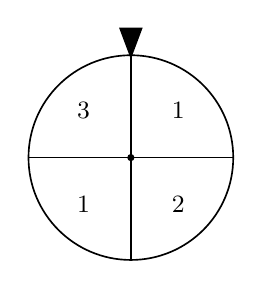
\begin{tikzpicture}[line width=0.6pt,baseline=(current bounding box.north)]\draw (0,0) circle (1.3);\draw (0,0) -- (90:1.3);\node[font=\small] at (45:0.85) {1};\draw (0,0) -- (0:1.3);\node[font=\small] at (-45:0.85) {2};\draw (0,0) -- (-90:1.3);\node[font=\small] at (-135:0.85) {1};\draw (0,0) -- (-180:1.3);\node[font=\small] at (-225:0.85) {3};\fill (0,0) circle (1.3pt);\fill (0,1.25) -- (-0.15,1.65) -- (0.15,1.65) -- cycle;\end{tikzpicture}\hspace{1.2cm}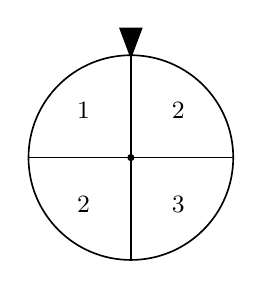
\begin{tikzpicture}[line width=0.6pt,baseline=(current bounding box.north)]\draw (0,0) circle (1.3);\draw (0,0) -- (90:1.3);\node[font=\small] at (45:0.85) {2};\draw (0,0) -- (0:1.3);\node[font=\small] at (-45:0.85) {3};\draw (0,0) -- (-90:1.3);\node[font=\small] at (-135:0.85) {2};\draw (0,0) -- (-180:1.3);\node[font=\small] at (-225:0.85) {1};\fill (0,0) circle (1.3pt);\fill (0,1.25) -- (-0.15,1.65) -- (0.15,1.65) -- cycle;\end{tikzpicture}\par
\pfzwfrage{Gib P(3 links) und P(3 rechts) an.}
\pfzwfrage{Berechne P(22).}
\rechenraster{3}
\fusshilfe{\mbox{66:~$\tfrac{1}{16}$; $\tfrac{1}{8}$ $\neq$ $\tfrac{1}{16}$}}
\end{pfnr}
\pfgruppe{}
\begin{pfnr}{P10 ’20}{67.}{3 BE}
Wirft man einen Würfel zweimal hintereinander, gibt es 36 verschiedene Augenpaare. Dabei zählen zum Beispiel (2,1) und (1,2) als verschiedene Ergebnisse. Max sagt: „Zwei gleiche Augenzahlen zu werfen ist wahrscheinlicher, als im ersten Wurf eine 6 zu werfen.“ Kreuze an:
\pfkreuzzeile{Max hat recht}\pfkreuzzeile{Max hat nicht recht. Begründe deine Entscheidung}
\pfzwfrage{Zähle die Augenpaare mit zwei gleichen Zahlen.}
\rechenraster{2}
\fusshilfe{\mbox{67:~Max hat nicht Recht; beide Wahrscheinlichkeiten $\tfrac{1}{6}$}}
\end{pfnr}
\pfgruppe{}
\begin{pfnr}{P10 ’25}{\llap{\textasteriskcentered\,}68.}{2 BE}
Bei einem Spiel werden zwei Scheiben gleichzeitig gedreht. Bleiben sie stehen, liest man an den Pfeilen erst die Ziffer der linken, dann die der rechten Scheibe ab. Im Bild entsteht so die Zahl 12. Alle Sektoren sind gleich groß. Bestimme die Wahrscheinlichkeit, eine 12 oder eine 21 zu drehen.
\par\smallskip\noindent 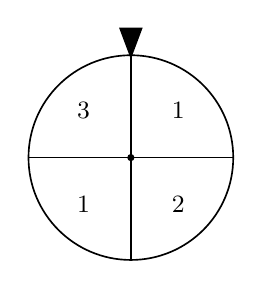
\begin{tikzpicture}[line width=0.6pt,baseline=(current bounding box.north)]\draw (0,0) circle (1.3);\draw (0,0) -- (90:1.3);\node[font=\small] at (45:0.85) {1};\draw (0,0) -- (0:1.3);\node[font=\small] at (-45:0.85) {2};\draw (0,0) -- (-90:1.3);\node[font=\small] at (-135:0.85) {1};\draw (0,0) -- (-180:1.3);\node[font=\small] at (-225:0.85) {3};\fill (0,0) circle (1.3pt);\fill (0,1.25) -- (-0.15,1.65) -- (0.15,1.65) -- cycle;\end{tikzpicture}\hspace{1.2cm}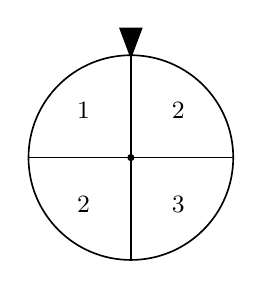
\begin{tikzpicture}[line width=0.6pt,baseline=(current bounding box.north)]\draw (0,0) circle (1.3);\draw (0,0) -- (90:1.3);\node[font=\small] at (45:0.85) {2};\draw (0,0) -- (0:1.3);\node[font=\small] at (-45:0.85) {3};\draw (0,0) -- (-90:1.3);\node[font=\small] at (-135:0.85) {2};\draw (0,0) -- (-180:1.3);\node[font=\small] at (-225:0.85) {1};\fill (0,0) circle (1.3pt);\fill (0,1.25) -- (-0.15,1.65) -- (0.15,1.65) -- cycle;\end{tikzpicture}\par
\rechenraster{3}
\fusshilfe{\mbox{68:~$\tfrac{5}{16}$ = 31,25 \%}}
\end{pfnr}
\pfgruppe{}
\begin{pfnr}{P10 ’14}{\llap{\textasteriskcentered\,}69.}{2 BE}
Für ein Kinderfest hat Pauls Vater ein Glücksrad gebaut. In einer Spielrunde wird es zweimal nacheinander gedreht. Alle Felder sind gleich groß und werden gleich wahrscheinlich getroffen. Berechne die Wahrscheinlichkeit, dass der Zeiger bei beiden Drehungen auf denselben Buchstaben zeigt.
\par\smallskip\noindent 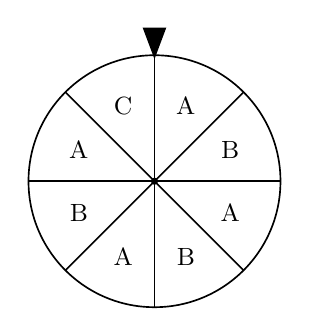
\begin{tikzpicture}[line width=0.6pt,baseline=(current bounding box.north)]\draw (0,0) circle (1.6);\draw (0,0) -- (90:1.6);\node[font=\small] at (67.5:1.04) {A};\draw (0,0) -- (45:1.6);\node[font=\small] at (22.5:1.04) {B};\draw (0,0) -- (0:1.6);\node[font=\small] at (-22.5:1.04) {A};\draw (0,0) -- (-45:1.6);\node[font=\small] at (-67.5:1.04) {B};\draw (0,0) -- (-90:1.6);\node[font=\small] at (-112.5:1.04) {A};\draw (0,0) -- (-135:1.6);\node[font=\small] at (-157.5:1.04) {B};\draw (0,0) -- (-180:1.6);\node[font=\small] at (-202.5:1.04) {A};\draw (0,0) -- (-225:1.6);\node[font=\small] at (-247.5:1.04) {C};\fill (0,0) circle (1.3pt);\fill (0,1.55) -- (-0.15,1.95) -- (0.15,1.95) -- cycle;\end{tikzpicture}\par
\rechenraster{3}
\fusshilfe{\mbox{69:~$\tfrac{13}{32}$ $\approx$ 0,41}}
\end{pfnr}
\pfstufekopf[sohnezurcklegen]{ohne Zurücklegen}{in 1 der letzten 5 Prüfungen}
\pfgruppe{}
\begin{pfnr}{eigene Aufgabe}{70.}{}
In einer Urne liegen 3 rote und 2 weiße Kugeln. Zwei werden ohne Zurücklegen gezogen. Wie groß ist die Wahrscheinlichkeit für zwei gleiche Farben?
\rechenraster{1}
\fusshilfe{\mbox{70:~$\tfrac{2}{5}$}}
\end{pfnr}
\begin{pfnr}{eigene Aufgabe}{\llap{\textasteriskcentered\,}71.}{2 BE}
In einem Hut liegen 7 Zettel für die Aufgaben einer Woche, auf einem steht „frei“. Tom zieht zuerst, dann zieht Lea aus den übrigen Zetteln. Wie groß ist die Wahrscheinlichkeit, dass Lea „frei“ zieht?
\rechenraster{1}
\fusshilfe{\mbox{71:~$\tfrac{1}{7}$}}
\end{pfnr}
\begin{pfnr}{eigene Aufgabe}{72.}{}
In einer Box liegen 9 Stifte, 4 davon grün. Drei Stifte werden ohne Zurücklegen gezogen. Wie groß ist die Wahrscheinlichkeit für drei grüne?
\rechenraster{1}
\fusshilfe{\mbox{72:~$\tfrac{1}{21}$}}
\end{pfnr}
\begin{pfnr}{eigene Aufgabe}{\llap{\textasteriskcentered\,}73.}{}
Beim Staffellauf wird die Reihenfolge der 9 Läuferinnen zufällig ausgelost; jede läuft genau einmal. Wie groß ist die Wahrscheinlichkeit, dass Pia unter den ersten drei ist?
\rechenraster{1}
\fusshilfe{\mbox{73:~$\tfrac{1}{3}$}}
\end{pfnr}
\begin{pfnr}{eigene Aufgabe}{\llap{\textasteriskcentered\,}74.}{3 BE}
In einer Kiste liegen 15 Stifte: 5 rote, 3 grüne und 7 schwarze. Drei Stifte werden ohne Zurücklegen gezogen. Leo behauptet: „Drei rote sind doppelt so wahrscheinlich wie drei grüne.“ Widerlege die Behauptung mit einer Rechnung.
\rechenraster{1}
\fusshilfe{\mbox{74:~zehnmal so wahrscheinlich, nicht doppelt}}
\end{pfnr}
\begin{pfnr}{eigene Aufgabe}{75.}{}
Bei einem Gewinnspiel liegen 5 Umschläge aus, in 2 steckt ein Gutschein. Du darfst zwei Umschläge öffnen. Wie groß ist die Wahrscheinlichkeit, mindestens einen Gutschein zu bekommen?
\rechenraster{1}
\fusshilfe{\mbox{75:~$0{,}7$}}
\end{pfnr}
\begin{pfnr}{P10 ’24}{\llap{\textasteriskcentered\,}76.}{2 BE}
In Familie Siebert helfen alle 5 Kinder im Haushalt. Jede Aufgabe steht auf einem Zettel: Müll rausbringen, Spülmaschine ausräumen, Staubsaugen, Einkaufen, Joker. Wer den Joker hat, hat die Woche frei. Zu Wochenbeginn zieht jedes Kind zufällig genau einen Zettel. Klara zieht immer als Zweite, direkt nach Benjamin. Ermittle, mit welcher Wahrscheinlichkeit Klara in Woche 1 den Joker bekommt.
\pfzwfrage{Gib an, mit welcher Wahrscheinlichkeit Benjamin den Joker nicht zieht.}
\pfzwfrage{Gib an, mit welcher Wahrscheinlichkeit Klara dann aus den vier übrigen Zetteln den Joker zieht.}
\rechenraster{2}
\fusshilfe{\mbox{76:~$\tfrac{1}{5}$}}
\end{pfnr}
\pfgruppe{}
\begin{pfnr}{P10 ’19}{\llap{\textasteriskcentered\,}77.}{3 BE}
In einer Kiste liegen 20 Buntstifte: 7 grüne, 4 rote, 3 gelbe und 6 blaue. Marc sagt: „Zieht man ohne Zurücklegen drei Stifte aus der Kiste, ist es doppelt so wahrscheinlich, drei blaue zu bekommen wie drei gelbe.“ Zeige mit einer Rechnung, dass Marc sich irrt.
\pfzwfrage{Berechne P(drei blaue).}
\rechenraster{3}
\fusshilfe{\mbox{77:~20-mal so hoch, Behauptung falsch}}
\end{pfnr}
\pfgruppe{}
\begin{pfnr}{P10 ’18}{\llap{\textasteriskcentered\,}78.}{4 BE}
Für ein anderes Fest backt Eva wieder 14 Pfannkuchen mit Marmelade (M) und 2 mit Senf (S). Der erste Gast nimmt blind nacheinander zwei Pfannkuchen. Er erwischt mindestens einen mit Senf: Nenne alle Ergebnisse, die dafür in Frage kommen. Ermittle die Wahrscheinlichkeit, dass beide Pfannkuchen des ersten Gastes Marmelade enthalten. Beschreibe in Worten das Ereignis E, dessen Wahrscheinlichkeit diese Rechnung angibt: $P(E) = \tfrac{2}{16}\cdot\tfrac{1}{15} + \tfrac{14}{16}\cdot\tfrac{13}{15}$
\rechenraster{3}
\fusshilfe{\mbox{78:~(S; M), (M; S), (S; S); $\approx$ 0,758}}
\end{pfnr}
\pfstufekopf[sgegenereignis]{Gegenereignis}{in 1 der letzten 5 Prüfungen}
\pfgruppe{}
\begin{pfnr}{eigene Aufgabe}{79.}{}
Ein Würfel wird einmal geworfen. Wie groß ist die Wahrscheinlichkeit, dass weder 2 noch 3 noch 4 fällt?
\rechenraster{1}
\fusshilfe{\mbox{79:~$\tfrac{1}{2}$}}
\end{pfnr}
\begin{pfnr}{eigene Aufgabe}{80.}{}
Ein Würfel wird zweimal geworfen. Wie groß ist die Wahrscheinlichkeit für mindestens eine 6?
\rechenraster{1}
\fusshilfe{\mbox{80:~$\tfrac{11}{36}$}}
\end{pfnr}
\pfgruppe{}
\begin{pfnr}{eigene Aufgabe}{\llap{\textasteriskcentered\,}81.}{2 BE}
Ein roter Würfel trägt die Zahlen 1, 2, 2, 3, 5, 6, ein blauer Würfel 2, 3, 3, 5, 5, 5. Erst wird der rote, dann der blaue geworfen. Wie groß ist die Wahrscheinlichkeit, dass nicht zweimal eine ungerade Zahl fällt?
\rechenraster{1}
\fusshilfe{\mbox{81:~$\tfrac{7}{12}$}}
\end{pfnr}
\pfstufekopf[szufallsgertentwerfen]{Zufallsgerät entwerfen}{in 2 der letzten 5 Prüfungen}
\pfgruppe{}
\begin{pfnr}{eigene Aufgabe}{82.}{1 BE}
Ein Glücksrad hat 4 gleich große Felder in Rot und Gelb. Die Wahrscheinlichkeit für Gelb ist 75\,\%. Wie viele Felder sind gelb?
\rechenraster{1}
\fusshilfe{\mbox{82:~$3$ Felder}}
\end{pfnr}
\begin{pfnr}{eigene Aufgabe}{83.}{}
Zeichne ein Glücksrad mit 6 gleich großen Feldern. Die Wahrscheinlichkeit für Rot soll $\tfrac{1}{2}$ sein, für Blau $\tfrac{1}{3}$. Die übrigen Felder sind gelb.
\par\smallskip\noindent \kreisleer[2]\par
\rechenraster{1}
\fusshilfe{\mbox{83:~3 rote, 2 blaue, 1 gelbes Feld}}
\end{pfnr}
\begin{pfnr}{eigene Aufgabe}{\llap{\textasteriskcentered\,}84.}{2 BE}
Das Bild zeigt zwei leere Glücksräder mit je vier gleich großen Feldern. Man liest erst das linke, dann das rechte Rad. Trage Ziffern so ein, dass die Wahrscheinlichkeit für 57 genau $\tfrac{3}{8}$ ist. Zeige es mit einer Rechnung.
\par\smallskip\noindent \kreisdiagramm{/1,/1,/1,/1} \kreisdiagramm{/1,/1,/1,/1}\par
\rechenraster{1}
\fusshilfe{\mbox{84:~$\tfrac{3}{8}$}}
\end{pfnr}
\begin{pfnr}{P10 ’18}{85.}{1 BE}
Ein Glücksrad hat 5 gleich große Felder in den Farben Rot, Grün und Weiß. Mit 40 \% Wahrscheinlichkeit bleibt es bei einmaligem Drehen auf Rot stehen. Gib an, wie viele Felder rot sind.
\rechenraster{1}
\fusshilfe{\mbox{85:~2 rote Felder}}
\end{pfnr}
\pfgruppe{}
\begin{pfnr}{P10 ’25}{\llap{\textasteriskcentered\,}86.}{2 BE}
Bei einem Spiel werden zwei Scheiben gleichzeitig gedreht. Bleiben sie stehen, liest man an den Pfeilen erst die Ziffer der linken, dann die der rechten Scheibe ab. Im Bild entsteht so die Zahl 12. Alle Sektoren sind gleich groß. Trag in die beiden leeren Scheiben Ziffern so ein, dass man mit 25 \% Wahrscheinlichkeit eine 13 dreht. Begründe deine Einträge mit einer Rechnung.
\par\smallskip\noindent \begin{tikzpicture}[line width=0.6pt,baseline=(current bounding box.north)]\draw (0,0) circle (1.3);\draw (0,0) -- (90:1.3);\draw[line width=0.4pt] ($(45:0.81)+(-0.25,-0.12)$) rectangle ++(0.5,0.32);\draw (0,0) -- (0:1.3);\draw[line width=0.4pt] ($(-45:0.81)+(-0.25,-0.12)$) rectangle ++(0.5,0.32);\draw (0,0) -- (-90:1.3);\draw[line width=0.4pt] ($(-135:0.81)+(-0.25,-0.12)$) rectangle ++(0.5,0.32);\draw (0,0) -- (-180:1.3);\draw[line width=0.4pt] ($(-225:0.81)+(-0.25,-0.12)$) rectangle ++(0.5,0.32);\fill (0,0) circle (1.3pt);\fill (0,1.25) -- (-0.15,1.65) -- (0.15,1.65) -- cycle;\end{tikzpicture}\hspace{1.2cm}\begin{tikzpicture}[line width=0.6pt,baseline=(current bounding box.north)]\draw (0,0) circle (1.3);\draw (0,0) -- (90:1.3);\draw[line width=0.4pt] ($(45:0.81)+(-0.25,-0.12)$) rectangle ++(0.5,0.32);\draw (0,0) -- (0:1.3);\draw[line width=0.4pt] ($(-45:0.81)+(-0.25,-0.12)$) rectangle ++(0.5,0.32);\draw (0,0) -- (-90:1.3);\draw[line width=0.4pt] ($(-135:0.81)+(-0.25,-0.12)$) rectangle ++(0.5,0.32);\draw (0,0) -- (-180:1.3);\draw[line width=0.4pt] ($(-225:0.81)+(-0.25,-0.12)$) rectangle ++(0.5,0.32);\fill (0,0) circle (1.3pt);\fill (0,1.25) -- (-0.15,1.65) -- (0.15,1.65) -- cycle;\end{tikzpicture}\par
\pfzwfrage{Schreibe 25 \% als Produkt zweier Wahrscheinlichkeiten.}
\rechenraster{2}
\fusshilfe{\mbox{86:~25 \%}}
\end{pfnr}
\pfgruppe{}
\begin{pfnr}{P10 ’19}{87.}{1 BE}
In einem Gefäß liegen schwarze und weiße Kugeln. Das Baumdiagramm zeigt, mit welcher Wahrscheinlichkeit man eine schwarze oder eine weiße Kugel zieht. Zeichne die fehlenden weißen Kugeln in das Gefäß.
\par\smallskip\noindent \begin{tikzpicture}[line width=0.6pt,baseline=(current bounding box.north)]\draw (0,1.6) -- (0,0) -- (1.9,0) -- (1.9,1.6);\fill (0.30,0.25) circle (0.17);\fill (0.70,0.25) circle (0.17);\fill (1.10,0.25) circle (0.17);\fill (1.50,0.25) circle (0.17);\draw (3,0.8) -- (4.6,1.5) node[right,font=\small] {schwarz};\draw (3,0.8) -- (4.6,0.1) node[right,font=\small] {weiß};\node[font=\scriptsize,fill=white,inner sep=1pt] at (3.8,1.35) {$\tfrac{2}{3}$};\node[font=\scriptsize,fill=white,inner sep=1pt] at (3.8,0.25) {$\tfrac{1}{3}$};\fill (3,0.8) circle (1.2pt);\end{tikzpicture}\par
\pfzwfrage{Gib an, wie viele Kugeln insgesamt im Gefäß liegen müssen.}
\rechenraster{2}
\fusshilfe{\mbox{87:~2 weiße Kugeln}}
\end{pfnr}
\pfpruefstein{P10 ’26}
\begin{pfnr}{}{}{}
Zwei Würfel sind mit Zahlen beschriftet. Würfel A trägt 1, 1, 2, 2, 4, 5; Würfel B trägt 1, 1, 2, 3, 3, 3. Die Abbildung zeigt ihre Netze.
\par\smallskip\noindent 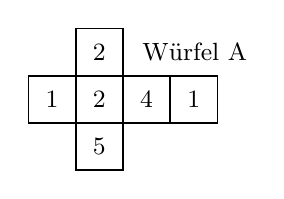
\begin{tikzpicture}[x=0.6cm,y=0.6cm,line width=0.6pt,baseline=(current bounding box.north)]\draw (1,2) rectangle ++(1,1); \node[font=\small] at (1.5,2.5) {2};\draw (0,1) rectangle ++(1,1); \node[font=\small] at (0.5,1.5) {1};\draw (1,1) rectangle ++(1,1); \node[font=\small] at (1.5,1.5) {2};\draw (2,1) rectangle ++(1,1); \node[font=\small] at (2.5,1.5) {4};\draw (3,1) rectangle ++(1,1); \node[font=\small] at (3.5,1.5) {1};\draw (1,0) rectangle ++(1,1); \node[font=\small] at (1.5,0.5) {5};\node[font=\small,anchor=south west] at (2.2,2.1) {Würfel A};\end{tikzpicture}\hspace{1cm}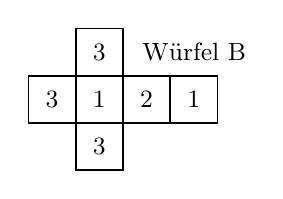
\begin{tikzpicture}[x=0.6cm,y=0.6cm,line width=0.6pt,baseline=(current bounding box.north)]\draw (1,2) rectangle ++(1,1); \node[font=\small] at (1.5,2.5) {3};\draw (0,1) rectangle ++(1,1); \node[font=\small] at (0.5,1.5) {3};\draw (1,1) rectangle ++(1,1); \node[font=\small] at (1.5,1.5) {1};\draw (2,1) rectangle ++(1,1); \node[font=\small] at (2.5,1.5) {2};\draw (3,1) rectangle ++(1,1); \node[font=\small] at (3.5,1.5) {1};\draw (1,0) rectangle ++(1,1); \node[font=\small] at (1.5,0.5) {3};\node[font=\small,anchor=south west] at (2.2,2.1) {Würfel B};\end{tikzpicture}\par
\end{pfnr}
\begin{pfnr}{}{a)}{1 BE}
Würfel A wird einmal geworfen. Gib die Wahrscheinlichkeit an, eine 2 zu würfeln.
\rechenplatz{3}
\end{pfnr}
\begin{pfnr}{}{b)}{4 BE}
Erst wird Würfel A geworfen, dann Würfel B. Man achtet nur darauf, ob die Zahl gerade oder ungerade ist. Ergänze die Wahrscheinlichkeiten im Baumdiagramm. Ermittle die Wahrscheinlichkeit, dass beide Würfel eine ungerade Zahl zeigen.
\par\smallskip\noindent \begin{tikzpicture}[line width=0.5pt,baseline=(current bounding box.north)]\node[font=\scriptsize,mbgrau] at (2.04,0.70) {Würfel A};\node[font=\scriptsize,mbgrau] at (5.44,0.70) {Würfel B};\fill (0,-1.35) circle (1.3pt) coordinate (k0w);\node[font=\scriptsize,inner sep=2pt] (k1) at (3.40,-2.25) {ungerade};\node[font=\scriptsize,inner sep=2pt] (k0) at (3.40,-0.45) {gerade};\node[font=\scriptsize,inner sep=2pt] (k2) at (6.80,0.00) {gerade};\node[font=\scriptsize,inner sep=2pt] (k3) at (6.80,-0.90) {ungerade};\node[font=\scriptsize,inner sep=2pt] (k4) at (6.80,-1.80) {gerade};\node[font=\scriptsize,inner sep=2pt] (k5) at (6.80,-2.70) {ungerade};\draw[] (k0w) -- node[pos=0.55,anchor=north,draw,line width=0.3pt,fill=white,minimum width=0.7cm,minimum height=0.34cm,inner sep=0pt] {} (k1.west);\draw[] (k0w) -- node[pos=0.55,anchor=south,font=\scriptsize,fill=white,inner sep=1pt] {$\tfrac{3}{6}$} (k0.west);\draw[] (k0.east) -- node[pos=0.55,anchor=south,font=\scriptsize,fill=white,inner sep=1pt] {$\tfrac{1}{6}$} (k2.west);\draw[] (k0.east) -- node[pos=0.55,anchor=north,draw,line width=0.3pt,fill=white,minimum width=0.7cm,minimum height=0.34cm,inner sep=0pt] {} (k3.west);\draw[] (k1.east) -- node[pos=0.55,anchor=south,draw,line width=0.3pt,fill=white,minimum width=0.7cm,minimum height=0.34cm,inner sep=0pt] {} (k4.west);\draw[] (k1.east) -- node[pos=0.55,anchor=north,draw,line width=0.3pt,fill=white,minimum width=0.7cm,minimum height=0.34cm,inner sep=0pt] {} (k5.west);\end{tikzpicture}\par
\rechenplatz{3}
\end{pfnr}
\begin{pfnr}{}{*c)}{2 BE}
Beide Würfel werden wie in b) geworfen. Bestimme die Wahrscheinlichkeit für das Ereignis E: „Nicht beide Würfel zeigen eine gerade Zahl.“
\rechenplatz{3}
\end{pfnr}
\begin{pfnr}{}{*d)}{2 BE}
Auf Würfel B wird genau eine Zahl geändert. Dann werden beide Würfel nacheinander geworfen. Beschrifte das leere Netz von Würfel B (neu) so, dass die Summe 2 mit der Wahrscheinlichkeit $\tfrac{1}{6}$ fällt. Zeige mit einer Rechnung, dass deine Beschriftung passt.
\par\smallskip\noindent 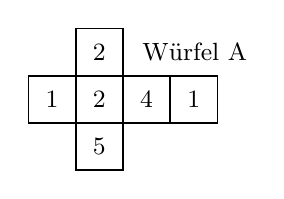
\begin{tikzpicture}[x=0.6cm,y=0.6cm,line width=0.6pt,baseline=(current bounding box.north)]\draw (1,2) rectangle ++(1,1); \node[font=\small] at (1.5,2.5) {2};\draw (0,1) rectangle ++(1,1); \node[font=\small] at (0.5,1.5) {1};\draw (1,1) rectangle ++(1,1); \node[font=\small] at (1.5,1.5) {2};\draw (2,1) rectangle ++(1,1); \node[font=\small] at (2.5,1.5) {4};\draw (3,1) rectangle ++(1,1); \node[font=\small] at (3.5,1.5) {1};\draw (1,0) rectangle ++(1,1); \node[font=\small] at (1.5,0.5) {5};\node[font=\small,anchor=south west] at (2.2,2.1) {Würfel A};\end{tikzpicture}\hspace{1cm}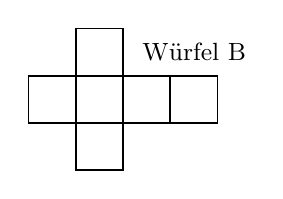
\begin{tikzpicture}[x=0.6cm,y=0.6cm,line width=0.6pt,baseline=(current bounding box.north)]\draw (1,2) rectangle ++(1,1); \node[font=\small] at (1.5,2.5) {};\draw (0,1) rectangle ++(1,1); \node[font=\small] at (0.5,1.5) {};\draw (1,1) rectangle ++(1,1); \node[font=\small] at (1.5,1.5) {};\draw (2,1) rectangle ++(1,1); \node[font=\small] at (2.5,1.5) {};\draw (3,1) rectangle ++(1,1); \node[font=\small] at (3.5,1.5) {};\draw (1,0) rectangle ++(1,1); \node[font=\small] at (1.5,0.5) {};\node[font=\small,anchor=south west] at (2.2,2.1) {Würfel B};\end{tikzpicture}\par
\rechenplatz{3}
\end{pfnr}
\end{document}